\documentclass[11pt,a4paper]{article}

\usepackage{amsmath}
\usepackage[version=3]{mhchem}
\usepackage[pdftex]{graphicx}

\setlength{\parindent}{0pt}

\title{CHEM210 \hfill Assignment 2}

\author{Mark Villar}

\begin{document}

\maketitle

\subsubsection*{Question 1}
	After calculating the number of valence electrons and drawing the Lewis dot structures of each molecule, we found the total regions of electron density by adding the number of 			bonded pairs (BP) and lone pairs (LP). The electronic and molecular geometries of each structure were then deduced. \\
	\begin{table}[!ht]
		\begin{center}
			\begin{tabular}{|c|c|c|c|c|c|}
				\hline
				 &Valence e$^{ -}$ &BP+LP &LP &Electronic &Molecular \\
				\hline
				\ce{ClO2^-} &20 &4 &2 &Tetrahedral &Bent  \\
				\ce{ClF4^+} &34 &5 &1 &Trigonal Bypyramid &Seesaw \\
				\ce{ICl4^-} &36 &6 &2 &Octahedral &Square Planar \\
				\ce{NF3} &26 &4 &1 &Tetrahedral &Trigonal Pyramid \\
				\ce{SO2} &16 &2 &0 &Linear &Linear \\
				\hline
			\end{tabular}
		\end{center}
	\end{table}

\subsubsection*{Question 2}
	\begin{table}[!ht]
		\begin{center}
			\begin{tabular}{|c|c|c|c|c|c|}
				\hline
				 &Valence e$^{ -}$ &BP+LP &LP &Electronic &Molecular \\
				\hline
				\ce{PF5} &40 &5 &0 &Trigonal Bypyramid &Trigonal Bypyramid  \\
				\ce{CH3I} &14 &4 &0 &Tetrahedral &Tetrahedral \\
				\ce{BrF5} &42 &6 &1 &Octahedral &Square Pyramid \\
				\hline
			\end{tabular}
		\end{center}
	\end{table}

	We would expect \ce{BrF5} to have bond angles that deviate from the ideal VSEPR values due to its single lone pair. Its molecular geometry is predicted to be square pyramidal, rather 			than the ideal octahedral structure.  As shown below, the  angles between bonded atoms are slightly less than 90$^\text{o}$.

\newpage 

	\begin{figure}[h]
		\centering
		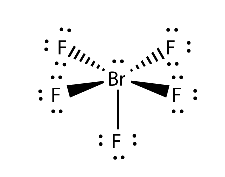
\includegraphics[width=4in]{BrF5.pdf}
	\end{figure}
	
	\begin{figure}[h]
		\centering
		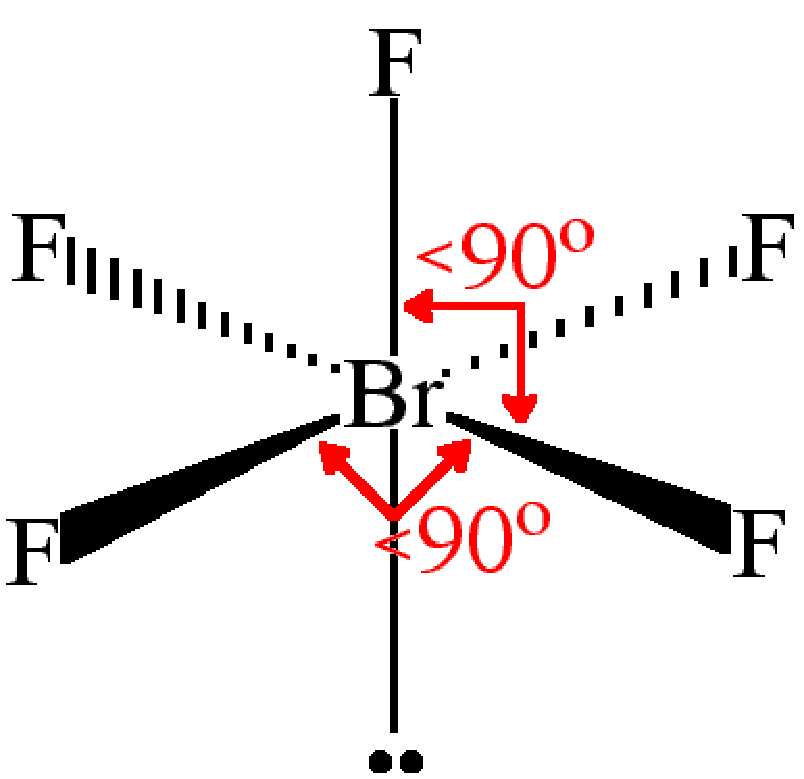
\includegraphics[width=3in]{BrF5_.pdf}
	\end{figure}

\newpage

\subsubsection*{Question 3}
	
\subsubsection*{Question 4}

\subsubsection*{Question 5} 

\subsubsection*{Question 6}

\subsubsection*{Question 7}

\subsubsection*{Question 8}  
	
\end{document}